\section{Architectural Constraints for Graph Processing: Locality}
\label{section:26-system-preliminaries}
Modern general-purpose architectures optimize for general-purpose computing. 
Most computing tasks involve working on a few key pieces of data for a long time or accessing data that are close to each other because we store things together that we will need to retrieve together. 
Graph processing does not resemble general-purpose computing, and so the architectural optimizations to capitalize on accessing data that are close together and reusing important data have a diminished impact.
Graphs lack locality.

\subsection{Locality}
Locality is a term in computer architecture that refers to the properties of data that enable it to be pre-emptively cached because it is nearby, and so is more likely to be needed than data that is far away (spatial locality) or is important and likely to be re-used soon (temporal locality).

\textbf{Spatial Locality.}
We store related data together and the idea of optimizing for spatial locality is that when data is needed for processing, data stored near it in memory is also likely to be needed for processing soon, so proximal memory blocks can be pre-emptively fetched to the cache for quick access~\cite{Hennessy2019}.
In figure~\ref{figure:locality-simple}, the vertices are stored in memory in \textit{vertex-order}, that is, written to memory in the order they are created (irrespective of edges).
% \nrscomment{cut next sentence}
% Assuming we can load a block of $3$ contiguous vertices at a time from memory to a simple single-level cache as an example, the benefit of exploiting \textit{spatial locality} is evident.
% In most BFS implementations, the vertices linked by outgoing edges from the source vertex (\textbf{A} for this example) are added to a queue, with each being processed in turn until the target vertex is found.
% \nrscomment{This isnt a terribly hard concept to understand,e specially if the figure is goo, i dont think you need to step through it in the prose}
% So, for the graph in figure~\ref{figure:locality-simple}, we would load the first three vertices from memory (\textbf{A, B} and \textbf{C}) to the cache for quick retrieval. 
% The first `expansion' of \textbf{A} enqueues the pointers to \textbf{B} and \textbf{F}.
% \textbf{B} is already in the cache and the `cache hit' when it is dequeued for expansion means that the vertex is quickly retrieved, exploiting the spatial locality of \textbf{A} and \textbf{B} in this instance. 
% The processor expands \textbf{B} to add the pointer to its neighbor \textbf{C} to the queue.
% When it comes time to expand \textbf{F}, however, there is a `cache miss'.
% \textbf{F} is not in the cache, so the processor must now wait for it to be loaded from main memory, incurring a penalty proportional to the latency of retrieving the vertex from main memory plus the time it takes to load the whole block given memory bandwidth constraints. 
% For simplicity, let us now assume that we have loaded another $3$ vertices starting from \textbf{F} (\textbf{F, G, H}) to replace the content of the cache and expand \textbf{F}, adding its neighbor \textbf{D} to the queue. 
% \textbf{C} is now at the front of the queue but has been bumped out of the cache by the load of (\textbf{F, G, H}) so the processor must wait again for \textbf{C} to be loaded from main memory before it can be expanded. 
% The problem continues throughout the algorithm, effectively `chasing pointers' all over the main memory, the `irregular memory accesses' that cause so much difficulty in graph processing~\cite{Beamer2015}.
% The `pointer chasing' behavior here happens because of the poor \textit{spatial locality} in this graph.
% \nrscomment{the below stuff is worth keeping, just make the second sentence more generic instead of referring to the example specific}
This manner of storage typically leads to a situation in which the vertices that are close to each other in the graph topologically are not close to each other in memory. 
In other words, they lack spatial locality.
The lack of spatial locality also means that only a small percentage of each cache line is used in each step as irrelevant information is retrieved just because it happens to be nearby.
The irregular memory access problem is exacerbated in larger graphs, where it is more likely that the vertex list does not fit in the cache and the processor will have to access the main memory to retrieve the data~\cite{Chung2012}, which is reflected empirically in a decreasing \textit{instructions per miss} rate on larger graphs~\cite{Beamer2015}.

%Rendering of the simplest possible Graph
\begin{figure}
    \begin{center}
        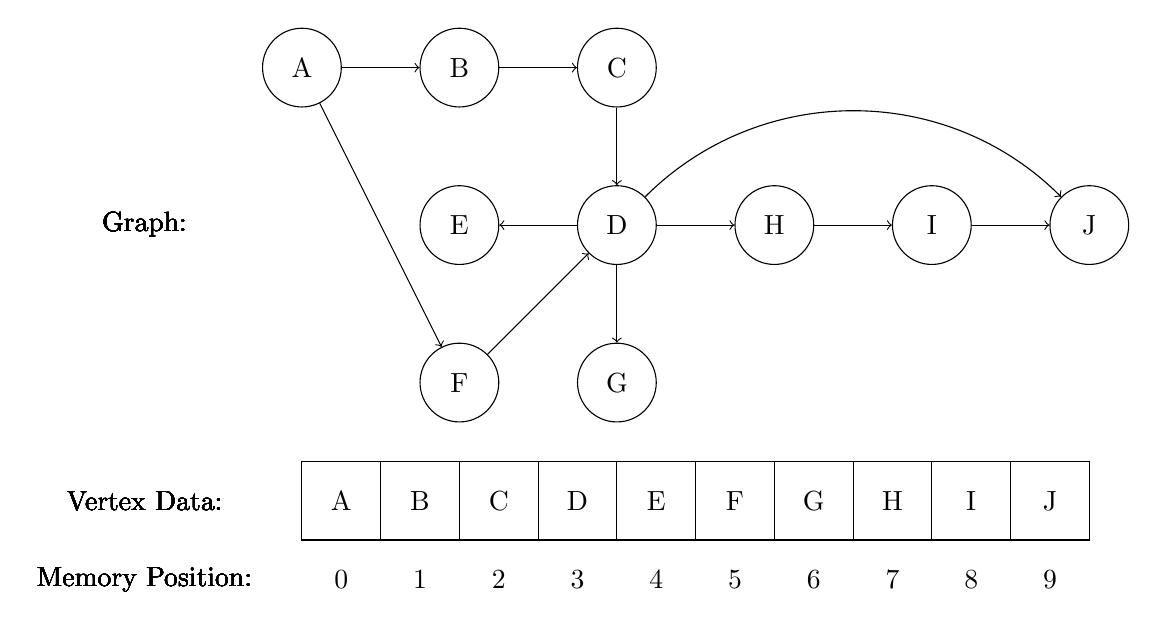
\begin{tikzpicture}

            % Graph vertices
            \node[circle,draw,minimum size=1cm] (A) at (0,0) {A};
            \node[circle,draw,minimum size=1cm] (B) at (2,0) {B};
            \node[circle,draw,minimum size=1cm] (C) at (4,0) {C};
            \node[circle,draw,minimum size=1cm] (D) at (4,-2) {D};
            \node[circle,draw,minimum size=1cm] (E) at (2,-2) {E};
            \node[circle,draw,minimum size=1cm] (F) at (2,-4) {F};
            \node[circle,draw,minimum size=1cm] (G) at (4,-4) {G};
            \node[circle,draw,minimum size=1cm] (H) at (6,-2) {H};
            \node[circle,draw,minimum size=1cm] (I) at (8,-2) {I};
            \node[circle,draw,minimum size=1cm] (J) at (10,-2) {J};
            
            % Graph Edges
             \draw[->] (A) -- (B);
             \draw[->] (A) -- (F);
             \draw[->] (B) -- (C);
             \draw[->] (C) -- (D);
             \draw[->] (D) -- (E);
             \draw[->] (F) -- (D);
             \draw[->] (D) -- (G);
             \draw[->] (D) -- (H);
             \draw[->] (D) to [out=45,in=135] (J);
             \draw[->] (H) -- (I);
             \draw[->] (I) -- (J);

            %Memory Array
             \foreach \x/\letter in {0/A, 1/B, 2/C, 3/D, 4/E, 5/F, 6/G, 7/H, 8/I, 9/J} {
                \draw (\x,-6) rectangle ++(1,1);
                \node at (\x+0.5, -5.5) {\letter};
                \node at (\x+0.5, -6.5) {\x};
            
            %Labels
            \node at (-2,-2) {Graph:};
            \node at (-2,-5.5) {Vertex Data:};
            \node at (-2,-6.5) {Memory Position:};
    }

            \end{tikzpicture}
        \caption{A simplified representation of a direct graph in vertex-order where each vertex is added to memory in the order it was created (here, alphabetically). Edges are not represented here.}
        \label{figure:locality-simple}          
    \end{center}
\end{figure}

\textbf{Temporal Locality.} 
We tend to transition between related tasks, so data that is important for what we are doing now is likely to be important for what we do next. 
Temporal locality is the idea that when a piece of data is needed for processing, it will likely be needed for processing again soon, so it can be retained in the cache for quick access.
To \textit{exploit} the \textit{temporal locality} systems can cache high-degree vertices since they are likely to be needed often~\cite{Beamer2015}.
% \nrscomment{id flip the order youre saying these things. first what is temporal locality -- the bit where high degree nodes are cached. Then talk about how this is especially useful for scale-free because xyz.}
There is some natural locality in \textit{scale-free} graphs that can be readily exploited. 
Consider figure~\ref{figure:locality-simple} again. 
While it is a very rudimentary sketch of a graph, vertex \textbf{D} has a much higher \textit{degree} than the other vertices. 
It is likely to be visited multiple times during processing, so caching it will reduce the number of times it needs to be pulled from memory.
% \nrscomment{is it really just based on the degree? from the name id think it would be a recency thing like with normal caching }

%Rendering of the simplest possible Graph
\begin{figure}
    \begin{center}
        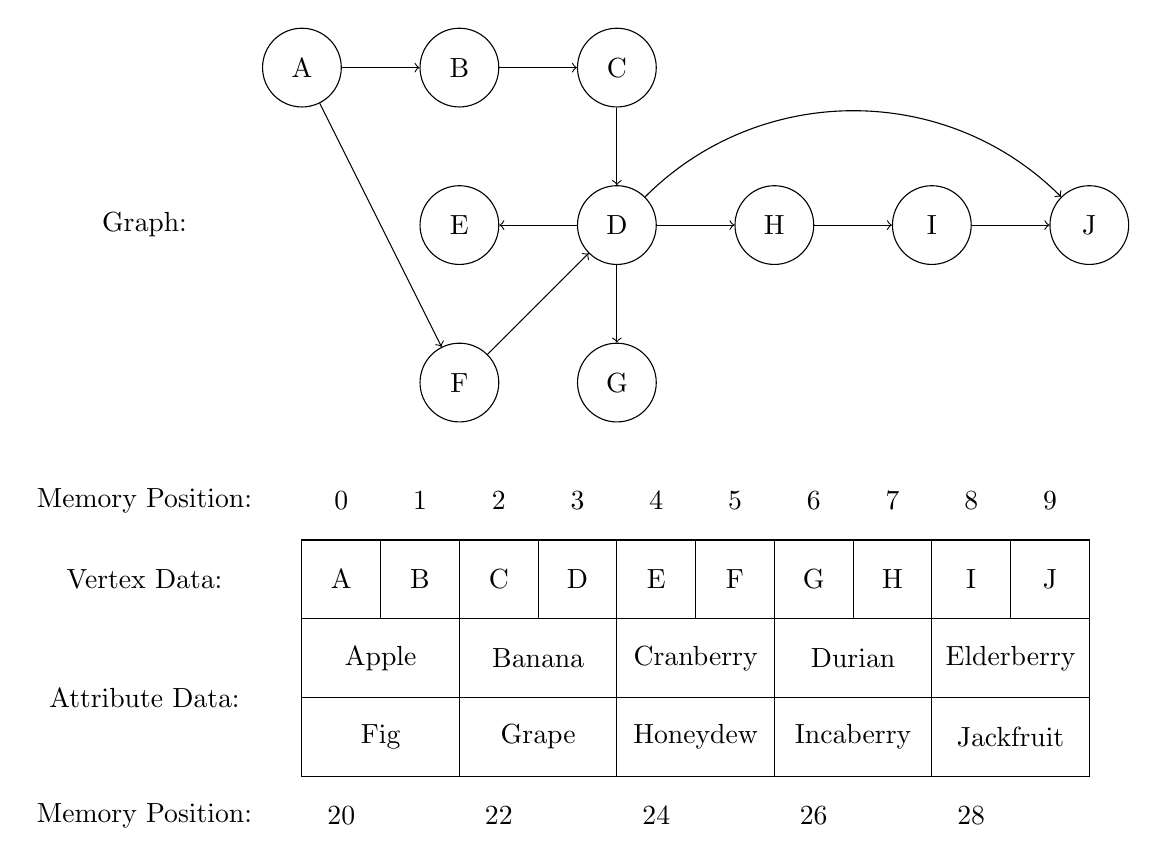
\begin{tikzpicture}

            % Graph vertices
            \node[circle,draw,minimum size=1cm] (A) at (0,0) {A};
            \node[circle,draw,minimum size=1cm] (B) at (2,0) {B};
            \node[circle,draw,minimum size=1cm] (C) at (4,0) {C};
            \node[circle,draw,minimum size=1cm] (D) at (4,-2) {D};
            \node[circle,draw,minimum size=1cm] (E) at (2,-2) {E};
            \node[circle,draw,minimum size=1cm] (F) at (2,-4) {F};
            \node[circle,draw,minimum size=1cm] (G) at (4,-4) {G};
            \node[circle,draw,minimum size=1cm] (H) at (6,-2) {H};
            \node[circle,draw,minimum size=1cm] (I) at (8,-2) {I};
            \node[circle,draw,minimum size=1cm] (J) at (10,-2) {J};
            
            % Graph Edges
             \draw[->] (A) -- (B);
             \draw[->] (A) -- (F);
             \draw[->] (B) -- (C);
             \draw[->] (C) -- (D);
             \draw[->] (D) -- (E);
             \draw[->] (F) -- (D);
             \draw[->] (D) -- (G);
             \draw[->] (D) -- (H);
             \draw[->] (D) to [out=45,in=135] (J);
             \draw[->] (H) -- (I);
             \draw[->] (I) -- (J);

            %Memory Array
             \foreach \x/\letter in {0/A, 1/B, 2/C, 3/D, 4/E, 5/F, 6/G, 7/H, 8/I, 9/J} {
                
                \node at (\x+0.5, -5.5) {\x};
                \draw (\x,-7) rectangle ++(1,1);
                \node at (\x+0.5, -6.5) {\letter};
                
             }

            %Attribute Array:

            \foreach \x/\attr in {0/Apple, 2/Banana, 4/Cranberry, 6/Durian, 8/Elderberry} {
                % \node at (\x,-8) {1\x};
                \draw (\x,-8) rectangle ++(2,1);
                \node at (\x+1,-7.5) {\attr};
            }
            \foreach \x/\attr in {0/Fig, 2/Grape, 4/Honeydew, 6/Incaberry, 8/Jackfruit}{
                \draw (\x,-9) rectangle ++(2,1);
                \node at (\x+1,-8.5) {\attr};
                \node at (\x+0.5,-9.5) {2\x};
            }
            
            %Labels
            \node at (-2,-2) {Graph:};
            \node at (-2,-5.5) {Memory Position:};
            \node at (-2,-6.5) {Vertex Data:};

            \node at (-2, -8) {Attribute Data:};
            \node at (-2, -9.5) {Memory Position:};


            \end{tikzpicture}
        \caption{A simplified representation of a directed graph in vertex order where each vertex is added to memory creation order with attributes stored separately. Pointers from topology to attributes are not shown for clarity but correspond to the first letter of the attribute.}
        \label{figure:locality-attributed}          
    \end{center}
\end{figure}

\textbf{Attributed Graphs and Locality.}
The latency problem is exacerbated by attributed graphs because graph attributes are often stored separately in memory~\cite{Buluc2013}. 
Figure~\ref{figure:locality-attributed} expands on the example from figure~\ref{figure:locality-simple} by adding in vertex attributes. 
The attributes are stored at separate memory locations, with pointers from the topological vertex (memory positions $1-9$) to their respective attributes (memory positions $10-29$). 
Attributes consume more memory, so more memory bandwidth is required to load them.
The heterogeneous data types being loaded in attributed graphs (like knowledge graphs) have been shown to increase the number of Dynamic Random Access Memory (DRAM) accesses and, hence, increase latency and memory bandwidth pressure~\cite{Basak2019}.
% \nrscomment{forget the example and just say either you have to check every vertex or you have to load the attributes too and fill up the cache that way}
To illustrate why, again consider a BFS that is searching for the `\textbf{Grape}' vertex. 
Each time a vertex is dequeued, its attribute must be retrieved from memory to see if it is the target vertex. 
In the worst case, this is a memory access each time a vertex is checked, or, if reducing the latency of the comparison by pre-fetching the attribute along with the vertex, the cache block of $3$ quickly becomes filled with the vertex plus its attribute, exacerbating the spatial locality problem.